
\chapter{函数图形}
\label{chap:graphs-of-functions}

\section{基本函数}
\label{sec:graphs-of-basic-functions}

\begin{itemize}
\item 一元一次函数

\begin{center}
  \begin{tikzpicture}[scale=1.0]
    \begin{scope}[shift={(0,0)}]
      \draw[|<->](-2,-.5)--(0,-.5)node[midway,below]{$\dfrac ba$};
      \draw[|<->](.5,1)--(.5,0)node[midway,right]{$b$};
      % \node[below] at (0,-2) {$y=ax+b$};
      \draw[->](-4,0)--(4,0) node[below]{$x$};
      \draw[->](0,-1)--(0,3) node[left]{$y$};
      \draw[very thick](-4,-1)--(4,3) node[below,right]{$f(x)=ax+b$};
    \end{scope}
  \end{tikzpicture}
\end{center}

\item 一元二次函数,其一般表达式(配方后)为
\begin{align*}
  f(x)=a\left(x+b\right)^2+c
\end{align*}
其对称轴为$x=-b$,唯一极值点为$(-b,c)$。
\begin{center}
  \begin{tikzpicture}[scale=2.0]
    \begin{scope}[shift={(0,0)}]
      \draw[->](-2,0)--(2,0) node[below]{$x$};
      \draw[->](0,-1)--(0,1.5) node[left]{$y$};
      \draw[dashed](.25,-1)--(.25,1.5) node[pos=0,right]{$x=-b$};
      \draw[dashed](-2,-.625)--(2,-.625) node[below]{$y=c$};
      \draw[very thick,domain=-.75:1.25,smooth,variable=\x]plot({\x},{2*\x*\x - \x - .5});
    \end{scope}
  \end{tikzpicture}
\end{center}

\item 三次方函数
\begin{center}
  \begin{tikzpicture}[scale=.5]
    \begin{scope}[shift={(0,0)}]
      \draw[->](-6,0)--(6,0) node[below]{$x$};
      \draw[->](0,-8)--(0,8) node[left]{$y$};
      \draw[very thick,domain=-2:2,smooth,variable=\x]plot({\x},{\x*\x*\x});
      \node[below right] at(1,1){$f(x)=x^3$};
    \end{scope}
  \end{tikzpicture}
\end{center}

\item 平方根函数
\begin{center}
  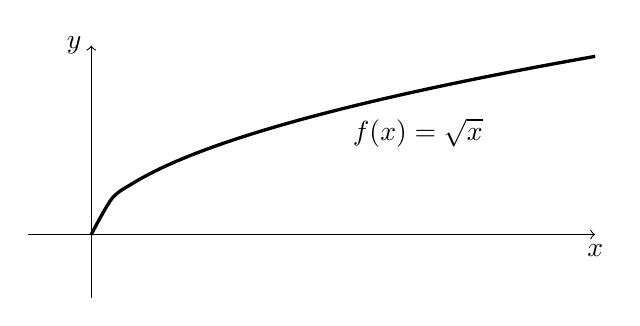
\begin{tikzpicture}[scale=.8]
    \begin{scope}[shift={(0,0)}]
      \draw[->](-1,0)--(8,0) node[below]{$x$};
      \draw[->](0,-1)--(0,3) node[left]{$y$};
      \draw[very thick,domain=0:8,smooth,variable=\x]plot({\x},{sqrt(\x)});
      \node[below right] at(4,2){$f(x)=\sqrt x$};
    \end{scope}
  \end{tikzpicture}
\end{center}

\item 绝对值函数
\begin{align*}
  f(x)=\left|x\right|=
  \begin{cases}
    -x,&\quad x<0\\
    \phantom{-}x,&\quad x\ge 0
  \end{cases}
\end{align*}
\begin{center}
  \begin{tikzpicture}[scale=1]
    \begin{scope}[shift={(0,0)}]
      \draw[->](-3,0)--(3,0) node[below]{$x$};
      \draw[->](0,-1)--(0,3.5) node[left]{$y$};
      \draw[very thick](-3,3)--(0,0)--(3,3) node[below right]{$f(x)=\left|x\right|$};
    \end{scope}
  \end{tikzpicture}
\end{center}

\item 倒数函数
\begin{center}
  \begin{tikzpicture}[scale=1]
    \begin{scope}[shift={(0,0)}]
      \draw[->](-3,0)--(3,0) node[below]{$x$};
      \draw[->](0,-3)--(0,3) node[left]{$y$};
      \draw[very thick,domain=.35:2.5,smooth,variable=\x]plot({\x},{1/\x});
      \draw[very thick,domain=-2.5:-.35,smooth,variable=\x]plot({\x},{1/\x});
      \node[right]at(1.1,1.5){$f(x)=\dfrac1x$};
    \end{scope}
  \end{tikzpicture}
\end{center}
\end{itemize}
